\section{Server Programming Language: \idx{Java}} % (fold)
\label{sec:java}

Nowadays, \idx{Java} is the most popular programming platform in corporative environments.
In \idx{ScaleNet} it is used in an \idx{OSGi} module that it is always running in the background providing real-time communication with the browser, besides a \idx{Java applet}.
In the end, no Java code was written for this project, since one of the goals was to move the files out of the \idx{OSGi} bundle to the \ida{PHP} scripts folder.

\subsection{History} % (fold)
\label{sub:javahistory}

\begin{wrapfigure}{r}{0.5\textwidth}
  \centering
    
\includegraphics[width=0.25\textwidth]{logo-java}
  \caption{\idx{Java} logo}
  \label{fig:logo-java}
\end{wrapfigure}

\emph{James Gosling} originally developed the language at \emph{Sun Microsystems} and released it to the public in 1995, within a initiative called \emph{Green Project} started in that company in 1991.

At first it was targeted at the digital cable television industry, but its true potential revealed to be the Internet, a much more dynamic platform.
It became rapidly popular for its promise of running anywhere, and even more after the most used browsers added support for \idx{Java applet}s.

The main difference with the existing languages was the \ida{JVM}.
It allowed to compile a program in an intermediate byte code that can run on any \idx{Java} supported device, independently of the underlying architecture.

In 1998 \idx{Java} 2 was released, with a \idx{Java} plugin and multiple versions targeted at different kind of scenarios (mobile devices, enterprise applications, limited devices, etc).
Since then every two years a new version was released until reaching \idx{Java} 6 in 2006, adding each time new capabilities to the language.

Starting in 2006, \emph{Sun} published Java's source code under the \ida{GPL}. Now, for the most part, it remains as free software and \emph{Oracle}, the current owner of the trademark, seems to be continuing the same strategy.

% subsection javahistory (end)

\subsection{Quick Overview of the Language} % (fold)
\label{sub:overviewjava}

According to \idx{Sun}\footnote{\url{http://java.sun.com/docs/white/langenv/Intro.doc2.html}}, there were five primary goals in the creation of the Java language:

\begin{itemize}
  \item It should be \emph{simple, object oriented, and familiar}.
  \item It should be \emph{robust and secure}.
  \item It should have \emph{an architecture-neutral and portable environment}.
  \item It should execute with \emph{high performance}.
  \item It should be \emph{interpreted, threaded, and dynamic}.
\end{itemize}

The syntax itself is very similar to \idx{C}, the main difference is that the code is organized around classes following \ida{OOP}.
By design it does not have any remarkable syntax anomaly, and the usual suspects are all there (if, for, while, etc).

It is strongly typed, and every variable needs to be declared with its type before using it.
Except the primitives types, everything is an object, which incidentally leads to an increased verbosity.

As said before, all code needs to be compiled.
The resulting byte code is not linked to any specific hardware, but to the \ida{JVM}.
This means that the compiled code is compatible with every supported platform, without any additional work, from a computer running Windows to a mobile phone.

The entry point for a \idx{Java} applications is the \idc{main} method of the main class.
The main class is usually declared outside of the \idx{Java} code in a manifest file.
The most common way of packaging a program is using a \ida{JAR} file, essentially just a \idx{ZIP} file containing the compiled code and a manifest.

All classes are organized in packages, each one focused in a different issue.
Like in \ida{PHP}, there is a lot of useful libraries already built in the \ida{JVM}, covering all the basic needs.
Due to its popularity, third party libraries are available for almost any imaginable problem.
To use any class outside of a package, the code needs to specifically import all the packages, even the bundled ones.

There is support for handling common problems and techniques, like threading, exceptions, user interfaces, security, networking, etc.
One of the most important features is its garbage collector, freeing the programmer from memory management tasks.

% subsection overviewjava (end)

\subsection{OSGi} % (fold)
\label{sub:osgi}

The \ida{OSGi} framework is a module system and service platform for \idx{Java} applications.
The main goal of this framework is providing a dynamic component model.
It offers a series of basic APIs to develop services, like logging, a \ida{HTTP} server and the \ida{DAS}, that eases the discovery of the device's capabilities.

An application or component developed for \ida{OSGi} is called a bundle, and it is a self-contained package with the compiled byte code, additional resources and a manifest.
According to that manifest, any bundle can be remotely installed, started, stopped, updated or uninstalled without requiring a reboot.
Figure~\vref{fig:osgi-layering} shows how bundles can interact with the framework and with each other.

\begin{figure}[htbp]
  \centering
    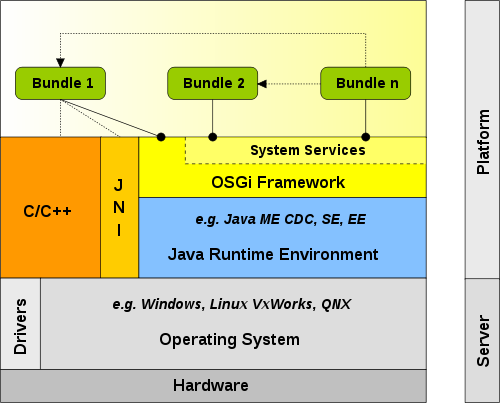
\includegraphics[width=0.85\textwidth]{osgi-layering}
  \caption{\idx{OSGi} layering}
  \label{fig:osgi-layering}
\end{figure}

The \ida{OSGi} specification is maintained by the \ida{OSGi} Alliance, backed by more than 35 big corporations and where \emph{Deutsche Telekom AG} acts as a full member.
There is also a vibrant open source community, having several open source implementations, for example this project uses \idx{Knopflerfish} \ida{OSGi}.
\ida{OSGi} R4 is the version used by this bundle, released originally in 2006 and currently the latest version available.

Once the framework is loaded, a console is available to manage all bundles.
Table~\vref{tab:osgicommands} lists the most used commands for that console.
This console will be running in the background all the time, so it may be useful to attach the process to a \idc{screen} process.

\begin{generictable}[\idx{OSGi} commands]{2}
  {|p{0.45\textwidth}|p{0.45\textwidth}|}
  {\generictitletwo{Command}{Description}}
  \label{tab:osgicommands}%
  \texttt{ps [-l | -s | -u]}           & List installed bundles. \\ \hline
  \texttt{refresh [<id> ...]}          & Refresh packages.       \\ \hline
  \texttt{install <URL> [<URL> ...]}   & Install bundle(s).      \\ \hline
  \texttt{uninstall <id> [<id> ...]}   & Uninstall bundle(s).    \\ \hline
  \texttt{start <id> [<id> <URL> ...]} & Start bundle(s).        \\ \hline
  \texttt{stop <id> [<id> ...]}        & Stop bundle(s).         \\ \hline
  \texttt{update <id> [<URL>]}         & Update bundle.          \\ \hline
  \texttt{shutdown}                    & Shutdown framework.     \\ \hline
\end{generictable}

In this framework modularity and portability are the key concepts.
This has proven useful in a wide range of fields like mobile phone, automobiles, grid computing, etc.
In this case it is used for building an application server, taking advantage of the built \ida{HTTP} server.

% subsection osgi (end)

\subsection{Java Applets} % (fold)
\label{sub:javaapplets}

A \idx{Java applet} is a small application written in \idx{Java} designed to be executed inside of a web browser, i.e., in the client machine.
An \idc{applet} \ida{HTML} tag (or the more recommendable \idc{object}) is embedded in the code specifying where the package is located, the dimensions that applet will occupy in the rendered page and the parameters that will receive.
Then the browser downloads it (distributed as a \ida{JAR} package), and executes it in the scope of that web page.

This enabled the development of interactive web applications with a much better performance than \idx{JavaScript} and more capabilities, while maintaining full compatibility within the supported platforms.
It was often used for graphic and resource-intensive applications, like plotting or basic gaming before Adobe Flash was popular.

Since it provides access to most of the \ida{JVM} classes, some web applications used them for functions not natively possible in a browser.
For example in this project a \idx{Java applet} is used solely for its native socket capabilities.

Security is critical in a platform like this that allows running code from the web with near-native privileges.
To alleviate this, by default an applet has very restricted access to the local filesystem and web pages.
The solution is to sign the applet with a trusted entity's certificate, relaxing those limitations.
In practice, this is an extra step that slows any iterative development and hardens deployments in corporative environments.

However, the rise of new standards and unsupported devices, the huge popularity of Adobe Flash, the qualitative improvements in \idx{JavaScript} performance and the disruptively poor user experience crippled its future and nowadays \emph{native} web alternatives are preferred over \idx{Java applet}s.

% subsection javaapplets (end)

% section java (end)
